\documentclass[10pt,a4paper]{article}
\usepackage{amsmath}   
\usepackage{graphicx}


\begin{document}
\section{Horizont Schätzung}
Aufgrund der \textit{2D-3D Transformation}, die im Kapitel \ref{sub:Pixel Transformation} vorgestellt wird, werden die Höhe und der Winkel der Horizontposition ebenfalls benötigt. Die Objekt Detektion liefert pro Zeitschritt drei Horizontkandidaten, die aufgrund Messungenauigkeiten, verzerrt sind. Die Ziele der Horizont Schätzung sind die Filterung der Messungen, um genauerer Ergebnisse zu erhalten und die Wahl des besten Kandidaten.\\
Die Filterung wird mithilfe des \textit{Kalman-Filters} durchgeführt und daher wird der ursprüngliche Zustand $\underline{x}_{k}$ auf 
\begin{equation}
\underline{x}^+_{k} = \begin{bmatrix}
\underline{x}_{k} \\
h_{k}\\
\alpha_{k}
\end{bmatrix}
\end{equation}
erweitert. Variablen $h_{k}$ und $\alpha_{k}$ stellen die Höhe beziehungsweise den Winkel des Horizonts dar.\\
Man geht von einem \textit{Constant Position Model} für den Horizont aus, das heißt:\\
\begin{equation}
h_k = h_{k-1}
\end{equation}
\begin{equation*}
\alpha_k = \alpha_{k-1},
\end{equation*}
was zu den System und Ausgangsmatrizen
\begin{equation}
\textbf{F}_{horizon} = \textbf{H}_{horizon} = \begin{bmatrix}
1 & 0  \\
0 & 1\\
\end{bmatrix}
\end{equation}
führt.\\
Die Anfangskovarianzmatrix des Systemfehlers $\textbf{P}_{0_{horizon}}$, die Varianz des Messrauschens $\textbf{R}_{horizon}$ und die Varianz des Systemrauschens $\textbf{Q}_{horizon}$ werden ebenfalls als eine zweidimensionale Einheitsmatrix angenommen.\\
Für den \textit{PHD} wird in dem ersten Zeitschritt $k = 0$ einen der drei Kandidaten einfach zufällig gewählt, da man keine zusätzliche Information verfügt, die diese Wahl beeinflussen kann.\\
Bei dem \textit{GNN} wird die Zeitverzögerung, die für den \textit{M/N Algorithmus} erforderlich ist, ausgenutzt, um bei $k = N$ den besten Kandidaten zu erhalten.
\section{Kandidatenermittlung für den \textit{GNN}}
	Mit den drei Horizontkandidaten, welche von der Objektdetektion zu jedem Zeitschritt geliefert werden, erhält man für die ersten N=4 Zeitschritte insgesamt zwölf Messpunkte über diesem Zeitraum verteilt. Abgesehen von der zeitlichen Abfolge, hat man keine Information darüber wie die Messpunkte untereinander verknüpft sind. Um trotzdem den besten Kandidaten zu ermitteln, wurden die Messpunkte miteinander über die zeitliche Abfolge kombiniert. Abbildung \ref{fig: Verteilung der Horizontkandidaten ueber die ersten N Zeitschritte} zeigt beispielhaft die Kombinationsmöglichkeiten. Bei drei Horizontkandidaten pro Zeitschritt und mit $N=4$ gibt es insgesamt $3^4=81$ Möglichkeiten die Messpunkte miteinander zu verknüpfen. Ausgehend von dem \textit{Constant Position Model} wurde die Kombination als bester Kandidat ausgewählt, welche die geringste Varianz aufwies.
	\begin{figure}[h]
		\centering
		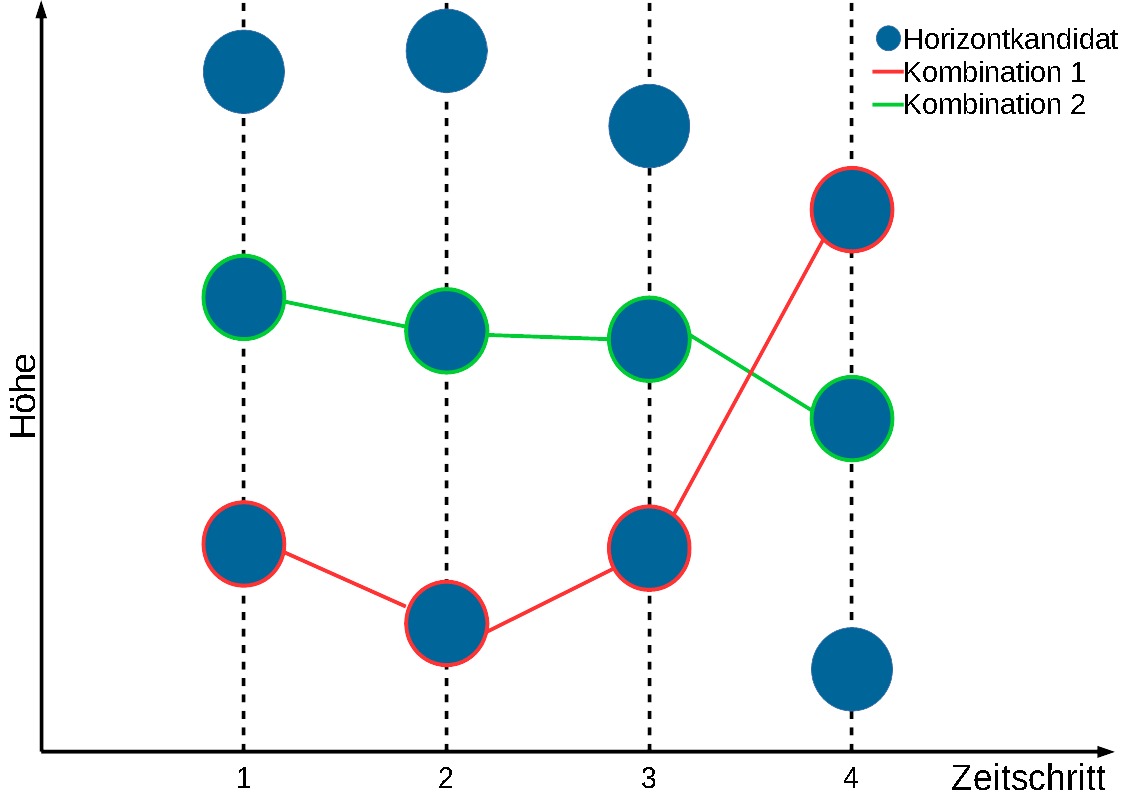
\includegraphics[width=.6\linewidth]{./Pictures_report/Verteilung der Horizontkandidaten ueber die ersten N Zeitschritte.png}
		\caption{Verteilung der  Horizontkandidaten über die ersten $N$ Zeitschritte}
		\label{fig: Verteilung der Horizontkandidaten ueber die ersten N Zeitschritte}
	\end{figure} 

\end{document}
